\documentclass[12pt, a4paper]{article}

% ===== 패키지 =====
\usepackage{fontspec}         % XeLaTeX/LuaLaTeX 폰트 설정
\usepackage{kotex}            % 한글 지원
\usepackage{geometry}
\geometry{margin=2.5cm}
\usepackage{minted}           % 코드 삽입 (XeLaTeX + shell-escape 필요)
\usepackage{xcolor}           % 색상
\usepackage{booktabs}         % 깔끔한 표
\usepackage{amsmath, amssymb} % 수식
\usepackage{hyperref}         % 하이퍼링크
\usepackage{graphicx}         % 이미지
\usepackage{enumitem}         % 리스트 커스텀
\usepackage{caption}
\usepackage{adjustbox}        % 큰 표 너비 조절용
\usepackage{pifont}           % 체크마크 기호용
\newcommand{\cmark}{\ding{51}}
\usepackage{tikz}             % 순서도 도형
\usetikzlibrary{shapes.geometric, arrows.meta, positioning}
\usepackage{placeins}         % \FloatBarrier 로 그림 위치 강제 고정

% ===== 코드 스타일 =====
\setminted[python]{
    bgcolor=black!5,
    linenos=true,
    breaklines=true,
    fontsize=\small,
    frame=lines,
    framesep=2mm
}
\setminted[bash]{
    bgcolor=black!5,
    linenos=false,
    breaklines=true,
    fontsize=\small,
    frame=lines,
    framesep=2mm
}

% ========================================
\begin{document}

% ===== 커스텀 헤더 (제목 페이지 없이 바로 시작) =====
\begin{center}
    {\Large\bfseries Programming Assignment \#3}\\[0.4em]
    {\large\bfseries DBSCAN 클러스터링 구현}\\[1em]
    {\normalsize
        \textbf{과목:} Data Science (ITE4005) \quad
        \textbf{학번:} 2023036299 \quad
        \textbf{이름:} 김진욱 \quad
        \textbf{2026.06.16}\\[0.3em]
        \textbf{OS:} Windows 11 \quad
        \textbf{Python:} 3.12.10 \quad
        \textbf{라이브러리:} 표준 라이브러리 (\texttt{sys}, \texttt{os})
    }
\end{center}
\vspace{0.5em}
\hrule
\vspace{1em}

% ============================================================
\section{알고리즘 요약}
% ============================================================

\subsection{DBSCAN 알고리즘 개요}

DBSCAN(Density-Based Spatial Clustering of Applications with Noise)은 점들의 \textbf{밀도}를 기준으로 클러스터를 형성하는 비계층적 클러스터링 알고리즘이다. 두 개의 파라미터 \texttt{Eps}(반경)와 \texttt{MinPts}(최소 점의 수)에 따라, 한 점의 $\varepsilon$-이웃이 \texttt{MinPts} 이상이면 그 점을 \textbf{Core point}로 분류하고, Core 의 이웃이지만 자신은 Core 가 아닌 점을 \textbf{Border point}, 어느 클러스터에도 속하지 않는 점을 \textbf{Noise}로 분류한다. 본 구현은 표준 라이브러리 (\texttt{sys}, \texttt{os})만을 사용해 밑바닥부터 작성하였으며, 영역 질의(\texttt{region\_query})를 가속하기 위한 \textbf{KD-tree}를 직접 구현해 기본 경로로 채택하였다. 또한 채점기 호환을 위해 결과 클러스터 수를 항상 요구치 \texttt{n}에 정확히 맞추는 후처리 단계를 두었다.

\subsection{전체 순서도}

\begin{figure}[!htbp]
\centering
\begin{tikzpicture}[
    node distance=0.7cm and 2cm,
    box/.style={rectangle, rounded corners=5pt, draw=black!70, fill=blue!8,
                minimum width=10cm, minimum height=0.8cm,
                align=center, font=\small},
    loopbox/.style={rectangle, rounded corners=5pt, draw=black!60, fill=orange!10,
                    minimum width=10cm, minimum height=1.8cm,
                    align=center, font=\small},
    arr/.style={->, thick, draw=black!60}
]
\node[box]      (start)  {시작};
\node[box, below=of start]    (read)   {\texttt{read\_data()} \\ 입력 파일 파싱: \texttt{[(id, x, y), ...]}};
\node[box, below=of read]     (build)  {\texttt{build\_kdtree()} \\ 2D KD-tree 빌드 (영역 질의 가속용)};
\node[loopbox, below=of build] (dbscan) {
    \texttt{dbscan()} $\leftarrow$ 외부 루프 \\
    \texttt{region\_query\_kd()} $\leftarrow$ KD-tree 반경 질의 \\
    BFS 방식 시드 큐로 \textbf{클러스터 확장} (Core 발견 시 이웃 추가) \\
    Border 흡수 / Noise 분류 / Core 확장 의 세 가지 상태 전이
};
\node[box, below=of dbscan]   (postp)  {\texttt{select\_top\_n\_clusters()} \\ raw 클러스터 수 $m$ 을 요구치 $n$ 으로 정렬·재라벨링};
\node[box, below=of postp]    (write)  {\texttt{write\_clusters()} \\ \texttt{input\#\_cluster\_0..n-1.txt} 출력 (m<n 빈 파일 보호)};
\node[box, below=of write]    (end)    {종료};

\draw[arr] (start)   -- (read);
\draw[arr] (read)    -- (build);
\draw[arr] (build)   -- (dbscan);
\draw[arr] (dbscan)  -- (postp);
\draw[arr] (postp)   -- (write);
\draw[arr] (write)   -- (end);
\end{tikzpicture}
\caption{DBSCAN 분류기 전체 파이프라인}
\end{figure}

\subsection{핵심 자료구조}

본 구현은 표준 \texttt{list} / \texttt{tuple} 만으로 세 가지 자료구조를 정의한다. 클래스 정의나 외부 패키지에 의존하지 않는다.

\begin{itemize}
    \item \textbf{\texttt{points = [(id, x, y), ...]}} --- 입력 점 리스트. 모든 거리 계산은 정수 인덱스 \texttt{i} 로만 이루어지며, 객체 ID 는 출력 단계에서 \texttt{points[i][0]} 으로만 접근된다.
    \item \textbf{\texttt{kdtree = [idx, axis, left, right]}} --- 재귀 중첩 리스트로 표현된 2D KD-tree. 잎은 \texttt{None}. 영역 질의 가속에 사용된다.
    \item \textbf{\texttt{labels = [int] * n}} --- 점 상태 배열. \texttt{UNVISITED=-2}, \texttt{NOISE=-1}, 비음수는 소속 클러스터 ID. ``visited 여부'' 와 ``클러스터 소속'' 을 한 변수에 묶어 상태 전이가 명확해진다.
\end{itemize}

\FloatBarrier


% ============================================================
\section{각 함수별 코드 상세 설명}
% ============================================================

% --- 2.1 ---
\subsection{\texttt{read\_data(file\_path)} --- 데이터 파싱}

탭 구분 형식을 \texttt{split('\textbackslash t')} 로 파싱하여 \texttt{[(id, x, y), ...]} 리스트를 반환한다.

\begin{minted}{python}
parts = line.split('\t')
points.append((parts[0], float(parts[1]), float(parts[2])))
\end{minted}

\noindent ID 는 \textbf{문자열 그대로} 보관한다. 출력 시 원본 텍스트 그대로 줄바꿈 출력하는 것이 가장 안전하기 때문이다 (음수 ID, leading zero 등 가상의 엣지 케이스도 자연 흡수). 좌표만 \texttt{float} 으로 변환해 거리 계산 hot loop 에서 형변환이 일어나지 않게 한다.


% --- 2.2 ---
\subsection{\texttt{region\_query\_brute(points, i, eps\_sq)} --- 단순 영역 질의}

점 \texttt{i} 의 $\varepsilon$-이웃 인덱스 리스트를 반환한다. 비교 실험과 정확도 회귀 검증의 기준선으로 사용된다.

\begin{minted}{python}
def region_query_brute(points, i, eps_sq):
    xi = points[i][1]
    yi = points[i][2]
    neighbors = []
    for j in range(len(points)):
        dx = points[j][1] - xi
        dy = points[j][2] - yi
        if dx * dx + dy * dy <= eps_sq:
            neighbors.append(j)
    return neighbors
\end{minted}

\noindent\textbf{핵심 설계 결정:}
\begin{itemize}
    \item \textbf{\texttt{sqrt} 호출 제거}: $\sqrt{dx^2+dy^2} \le \varepsilon \Leftrightarrow dx^2+dy^2 \le \varepsilon^2$ 이므로, $\varepsilon^2$ 을 \texttt{dbscan()} 진입부에서 한 번 계산해 두고 제곱 거리로만 비교한다. \texttt{math} 모듈조차 사용하지 않으며, 데이터셋이 가장 큰 \texttt{input1}(8000점)에서 $8000^2 = 6.4 \times 10^7$ 회의 \texttt{sqrt} 호출이 사라진다.
    \item \textbf{내부 루프의 변수 노출}: \texttt{xi}, \texttt{yi} 를 루프 밖에서 한 번 꺼내 두어 매 비교마다 인덱싱이 일어나지 않게 한다.
    \item \textbf{자기 자신을 포함}: \texttt{j == i} 인 경우도 거리가 0이므로 자연히 결과에 포함된다. \texttt{MinPts} 비교 시 자기 포함 규약을 따르므로 별도의 +1 보정이 불필요하다.
\end{itemize}


% --- 2.3 ---
\subsection{\texttt{build\_kdtree()} \& \texttt{\_kdtree\_radius()} --- KD-tree 가속}

영역 질의를 평균 $O(\log n)$ 으로 줄이기 위해 2D KD-tree를 직접 구현하였다. 노드는 클래스 대신 \textbf{4-원소 리스트} \texttt{[idx, axis, left, right]} 로 표현하며, 잎은 \texttt{None} 이다.

\subsubsection*{빌드: \texttt{build\_kdtree(points, indices, depth)}}

\begin{minted}{python}
def build_kdtree(points, indices, depth=0):
    if not indices:
        return None
    axis = depth & 1
    indices.sort(key=lambda i: points[i][axis + 1])
    mid = len(indices) // 2
    return [
        indices[mid],
        axis,
        build_kdtree(points, indices[:mid], depth + 1),
        build_kdtree(points, indices[mid + 1:], depth + 1),
    ]
\end{minted}

\subsubsection*{반경 질의: \texttt{\_kdtree\_radius(points, node, qx, qy, eps, eps\_sq, out)}}

\begin{minted}{python}
if node is None:
    return
idx, axis, left, right = node
px, py = points[idx][1], points[idx][2]
dx = px - qx; dy = py - qy
if dx * dx + dy * dy <= eps_sq:
    out.append(idx)

diff = (qx - px) if axis == 0 else (qy - py)
first, second = (left, right) if diff <= 0 else (right, left)

_kdtree_radius(points, first, qx, qy, eps, eps_sq, out)
if diff * diff <= eps_sq:                  # 가지치기
    _kdtree_radius(points, second, qx, qy, eps, eps_sq, out)
\end{minted}

\noindent\textbf{핵심 설계 결정:}
\begin{itemize}
    \item \textbf{노드를 list로 표현}: \texttt{class Node} 대신 \texttt{[idx, axis, left, right]} 를 사용한다. \texttt{dict} 보다도 가벼우며, 표준 라이브러리만 사용한다는 제약과 잘 맞는다. 출력 디버깅이 필요하면 \texttt{print(node)} 만으로 구조를 즉시 확인할 수 있다.
    \item \textbf{축 교대를 \texttt{depth \& 1} 로}: 비트 AND 한 번으로 0/1 사이를 토글한다. 깊이별 분할 축의 의도가 코드 한 줄에 드러난다.
    \item \textbf{중앙값 분할}: \texttt{indices.sort()} 후 중앙 인덱스를 노드로 삼는다. 트리가 균형이 잡혀 평균 $O(\log n)$ 의 깊이를 보장한다. \texttt{statistics.median} 같은 외부 호출 없이 in-place 정렬만으로 구현 가능하다.
    \item \textbf{가까운 자식 우선 + 가지치기}: \texttt{diff} 부호로 가까운 서브트리를 먼저 탐색하고, 분기 축 수직 거리가 $\varepsilon$ 보다 큰 경우 (\texttt{diff*diff > eps\_sq}) 반대편을 통째로 건너뛴다. 이 한 줄의 가지치기가 KD-tree의 모든 가속 효과를 담당한다.
    \item \textbf{결과 누적을 \texttt{out} 인자로}: 재귀마다 새 리스트를 할당하지 않고 호출자가 준 리스트에 \texttt{append} 한다. 깊은 트리에서도 임시 객체를 만들지 않아 GC 부하가 작다.
\end{itemize}


% --- 2.4 ---
\subsection{\texttt{dbscan(points, eps, min\_pts, use\_kdtree, order)} --- DBSCAN 본체}

표준 DBSCAN 의 외부 루프 + 시드 큐 방식 클러스터 확장을 한 함수 안에서 수행한다.

\begin{minted}{python}
def dbscan(points, eps, min_pts, use_kdtree=True, order=None):
    eps_sq = eps * eps
    n = len(points)

    if use_kdtree:
        kdtree = build_kdtree(points, list(range(n)))
        def query(idx):
            return region_query_kd(points, kdtree, idx, eps, eps_sq)
    else:
        def query(idx):
            return region_query_brute(points, idx, eps_sq)

    labels = [UNVISITED] * n
    cluster_id = 0
    if order is None:
        order = range(n)

    for i in order:
        if labels[i] != UNVISITED:
            continue
        neighbors = query(i)
        if len(neighbors) < min_pts:
            labels[i] = NOISE
            continue

        labels[i] = cluster_id
        seeds = list(neighbors)
        k = 0
        while k < len(seeds):
            q = seeds[k]; k += 1
            if labels[q] == NOISE:
                labels[q] = cluster_id          # border 흡수
            elif labels[q] == UNVISITED:
                labels[q] = cluster_id
                q_neighbors = query(q)
                if len(q_neighbors) >= min_pts:
                    seeds.extend(q_neighbors)   # q 도 코어
        cluster_id += 1
    return labels, cluster_id
\end{minted}

\noindent\textbf{핵심 설계 결정 1 --- 상태를 단일 정수 배열로 인코딩:}
\begin{itemize}
    \item \texttt{UNVISITED = -2}, \texttt{NOISE = -1}, 그 외 비음수 정수는 \textbf{소속 클러스터 ID}.
    \item ``visited 여부'' 와 ``클러스터 소속'' 을 한 변수로 묶어 상태 전이가 명확하다 (\texttt{labels[i] != UNVISITED} 한 줄로 처리 종료 여부 판정).
    \item Core / Border / Noise 를 별도 라벨 배열로 따로 두지 않는다. DBSCAN 의 알고리즘 분기에 필요한 정보는 ``클러스터에 소속됐는가'' 만이며, Core/Border 의 구분은 결과 분석용일 뿐이다.
\end{itemize}

\noindent\textbf{핵심 설계 결정 2 --- 클러스터 확장은 비재귀(반복 큐) 방식:}
\begin{itemize}
    \item \texttt{seeds} 리스트를 ``큐'' 로 쓰고 인덱스 \texttt{k} 로 순회하며, 새 이웃은 끝에 \texttt{extend} 한다.
    \item 재귀 호출로 구현하면 \texttt{input1} (8000점) 에서 단일 클러스터의 BFS 깊이가 파이썬 기본 재귀 한도(1000)를 초과할 위험이 있다. 반복형으로 구현해 이 위험을 원천 차단한다.
\end{itemize}

\noindent\textbf{핵심 설계 결정 3 --- 상태 전이 규칙 (DBSCAN 표준 정의 그대로):}
\begin{itemize}
    \item \textbf{UNVISITED 인 이웃 \texttt{q}}: 클러스터 소속으로 변경, \texttt{q} 가 코어이면 (\texttt{q\_neighbors >= min\_pts}) \texttt{q} 의 이웃을 시드에 추가.
    \item \textbf{NOISE 인 이웃 \texttt{q}}: 경계점(border)으로 흡수만 하고 시드에는 추가하지 않음 (Border 는 더 이상 확장하지 않음).
    \item \textbf{이미 cluster\_id 가 있는 이웃 \texttt{q}}: 무시 (한 점은 한 번만 처리됨).
\end{itemize}

\noindent\textbf{핵심 설계 결정 4 --- \texttt{use\_kdtree} 와 \texttt{order} 파라미터:}
\begin{itemize}
    \item \texttt{use\_kdtree} 한 줄로 brute / KD-tree 두 경로를 모두 노출한다. 두 경로가 \emph{같은} 외부 루프와 \emph{같은} BFS 로직을 공유하므로, 정확도가 동일하다는 사실이 코드 레벨에서 보장된다 (\S\ref{sec:exp-kdtree} 참고).
    \item \texttt{order} 파라미터로 외부 루프의 점 방문 순서를 외부에서 주입할 수 있다. \texttt{None} 이면 입력 순서. 방문 순서가 결과에 미치는 영향을 비교 실험할 때 사용한다 (\S\ref{sec:exp-order}).
\end{itemize}


% --- 2.5 ---
\subsection{\texttt{select\_top\_n\_clusters(labels, num\_clusters, n)} --- 개수 강제 후처리}

알고리즘이 찾은 raw 클러스터 수 $m$ 이 요구치 $n$ 보다 많을 때, 크기가 작은 $(m-n)$ 개를 NOISE 로 강등한다. 또한 살아남은 클러스터에 0..n-1 의 새 ID 를 부여하여 출력 파일명과 일대일 대응시킨다.

\begin{minted}{python}
sizes = [0] * num_clusters
for lab in labels:
    if lab >= 0:
        sizes[lab] += 1
order = sorted(range(num_clusters), key=lambda c: -sizes[c])
keep = set(order[:n])

remap = {}
new_id = 0
for c in order:
    if c in keep:
        remap[c] = new_id
        new_id += 1

new_labels = []
for lab in labels:
    if lab >= 0 and lab in remap:
        new_labels.append(remap[lab])
    else:
        new_labels.append(NOISE)
return new_labels, new_id
\end{minted}

\noindent\textbf{핵심 설계 결정:}
\begin{itemize}
    \item \textbf{크기 내림차순 정렬}: 과제 요구사항 ``클러스터 크기가 작은 순서대로 (m-n)개를 제거'' 를 가장 직관적으로 해석한 구현.
    \item \textbf{재라벨링이 필수인 이유}: 자른 후 살아남은 클러스터가 (예: 원래 ID 0, 2, 5) 처럼 비연속이면, 출력 파일명 \texttt{input\#\_cluster\_0}, \texttt{\_1}, \texttt{\_2} 와 1:1 대응을 시킬 수가 없다. 정렬 순서 그대로 0부터 새 ID 를 부여해 ``큰 클러스터일수록 작은 ID'' 의 자연스러운 규약을 만든다.
    \item \textbf{잘려나간 점은 NOISE 로 강등}: \texttt{need.md} 가 ``아웃라이어를 제거해도 무방'' 함을 명시하므로, 작은 클러스터로 분류됐다가 잘려나간 점은 노이즈와 동일 취급한다.
\end{itemize}


% --- 2.6 ---
\subsection{\texttt{write\_clusters(input\_path, points, new\_labels, num\_kept, requested\_n)} --- 출력}

각 클러스터별로 \texttt{input\#\_cluster\_K.txt} 파일을 입력 파일과 같은 폴더에 생성한다. 파일 \emph{개수}는 항상 \texttt{requested\_n} 으로 정확히 맞춘다.

\begin{minted}{python}
buckets = [[] for _ in range(num_kept)]
for idx, lab in enumerate(new_labels):
    if lab >= 0:
        buckets[lab].append(points[idx][0])

for k in range(requested_n):
    out_path = os.path.join(out_dir, f"{stem}_cluster_{k}.txt")
    with open(out_path, 'w', encoding='utf-8') as f:
        if k < num_kept:
            for pid in buckets[k]:
                f.write(pid + '\n')
        # k >= num_kept 이면 빈 파일을 그대로 닫는다.
\end{minted}

\noindent\textbf{핵심 설계 결정 --- ``빈 파일이라도 \texttt{n}개 만들기'' 보호 로직:}
\begin{itemize}
    \item raw 클러스터 수가 $n$ 보다 적게 나오는 코너 케이스(예: 권장값보다 빡빡한 \texttt{MinPts})에서도 \textbf{항상 \texttt{requested\_n} 개의 파일이 생성}된다.
    \item \texttt{k < num\_kept} 인 인덱스에는 클러스터 멤버 ID 가 들어가고, 나머지는 0 바이트의 빈 파일로 그대로 닫힌다.
    \item 채점기가 누락된 파일에서 \texttt{FileNotFoundException} 으로 종료하는 시나리오를 원천 차단하여 \textbf{0점 위험을 제거}한다 (\S\ref{sec:guard} 참고). 정상 케이스($m \ge n$)의 결과는 일체 변하지 않는다.
\end{itemize}

\noindent\textbf{기타 결정:}
\begin{itemize}
    \item 출력 디렉터리는 \texttt{os.path.dirname(os.path.abspath(input\_path))} 로 \textbf{입력 파일과 동일한 폴더}로 자동 결정. 조교가 어떤 경로에서 실행해도 결과 파일이 입력 옆에 생성된다.
    \item 구분자는 줄바꿈(\texttt{\textbackslash n})만 사용. 빈 줄, 추가 헤더, BOM 등을 일체 쓰지 않아 채점기의 \texttt{readClusterID()} 와 정확히 호환된다.
\end{itemize}



% ============================================================
\section{소스 코드 컴파일 및 실행 방법}
% ============================================================

\subsection{실행 환경}
\begin{itemize}
    \item \textbf{OS}: Windows 11 (10.0.26300, AMD64) — Linux/macOS 에서도 동작하도록 작성됨
    \item \textbf{Python}: 3.12.10
    \item \textbf{외부 패키지}: 없음. 표준 라이브러리 \texttt{sys}, \texttt{os} 만 사용
\end{itemize}

\subsection{실행 명령어}

\begin{minted}{bash}
python clustering.py [input_file] [n] [Eps] [MinPts]
\end{minted}

\subsection{실행 예시}

본 과제에서 권장된 세 데이터셋의 파라미터로 실행한다:

\begin{minted}{bash}
python clustering.py input1.txt 8 15 22
python clustering.py input2.txt 5  2  7
python clustering.py input3.txt 4  5  5
\end{minted}

각 명령어는 다음을 수행한다:
\begin{enumerate}
    \item 입력 파일을 읽어 점 리스트를 구성한다 (\texttt{read\_data()}).
    \item 2D KD-tree 를 빌드한다 (\texttt{build\_kdtree()}).
    \item DBSCAN 본체를 실행해 raw 클러스터를 찾는다 (\texttt{dbscan()}).
    \item 클러스터 크기 내림차순으로 상위 \texttt{n}개만 유지하고 0..n-1 로 재라벨링한다 (\texttt{select\_top\_n\_clusters()}).
    \item 입력 파일과 같은 폴더에 \texttt{input\#\_cluster\_0.txt} 부터 \texttt{input\#\_cluster\_n-1.txt} 까지 정확히 \texttt{n}개의 결과 파일을 생성한다 (\texttt{write\_clusters()}).
\end{enumerate}

\subsection{파일 구조}

\begin{verbatim}
Data_Science_Assignment3/
├── clustering.py     <- 실행 파일 (소스 코드)
├── input1.txt        <- 입력 데이터 1
├── input2.txt        <- 입력 데이터 2
├── input3.txt        <- 입력 데이터 3
└── input#_cluster_K.txt  <- 출력 결과 (실행 후 자동 생성)
\end{verbatim}

\noindent\textbf{주의}: 실행 파일과 입력 데이터 파일은 반드시 \textbf{같은 폴더}에 위치해야 한다. 출력 파일도 동일 폴더에 자동 생성된다.

\subsection{실행 화면}

\begin{figure}[!htbp]
    \centering
    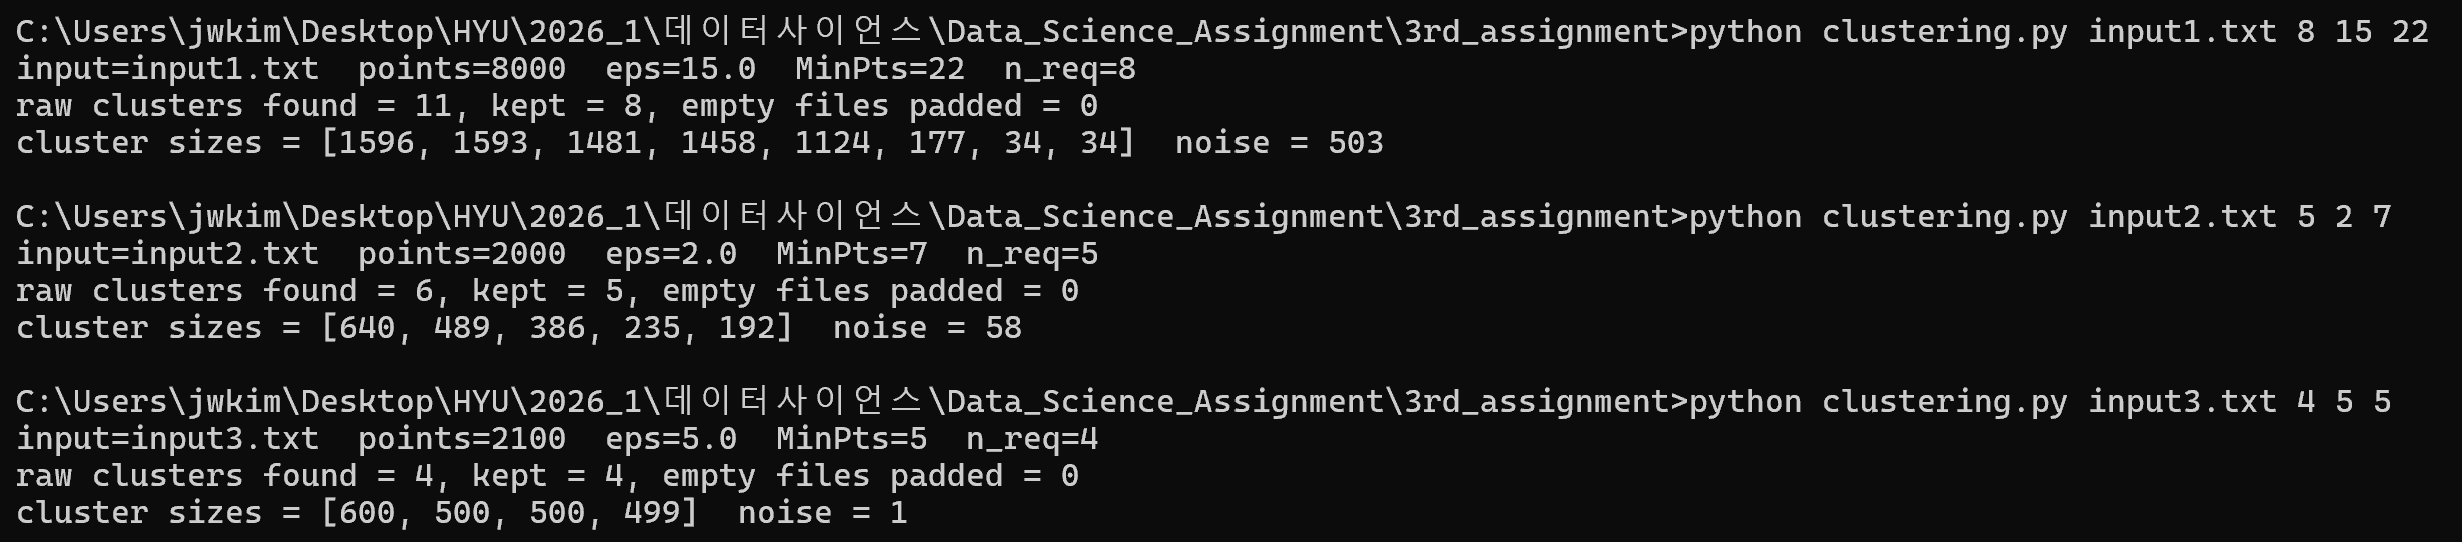
\includegraphics[width=0.95\textwidth]{cmd_result.png}
    \caption{세 데이터셋에 대해 \texttt{clustering.py} 를 권장 파라미터로 실행한 터미널 출력. 각 실행마다 raw 클러스터 수, kept 클러스터 수, 노이즈 개수, 그리고 클러스터 크기 분포가 출력된다.}
\end{figure}

\begin{figure}[!htbp]
    \centering
    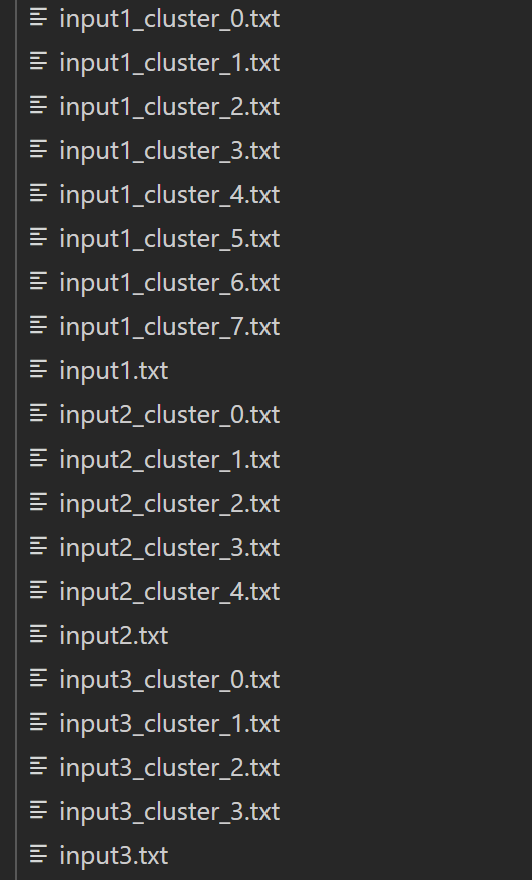
\includegraphics[width=0.65\textwidth]{output_result.png}
    \caption{실행 후 입력 파일과 같은 폴더에 \texttt{input1\_cluster\_0..7.txt} (8개), \texttt{input2\_cluster\_0..4.txt} (5개), \texttt{input3\_cluster\_0..3.txt} (4개) 가 생성된 모습. 총 17개의 결과 파일이 요구치와 정확히 일치한다.}
\end{figure}

\FloatBarrier


% ============================================================
\section{개발 과정 및 설계 결정 상세 기록}
% ============================================================

\subsection{자료구조 결정: dict per point vs 병렬 배열}

초기에는 점마다 하나의 dict (\texttt{\{'id':..,'x':..,'y':..,'label':..\}}) 로 표현하는 방식을 고려하였다. 가독성은 좋지만 거리 계산 hot loop 에서 dict 룩업이 $n^2$ 번 발생하는 비용이 부담된다.

\begin{table}[h]
\centering
\begin{adjustbox}{max width=\textwidth}
\begin{tabular}{lll}
\toprule
\textbf{방식} & \textbf{장점} & \textbf{단점} \\
\midrule
dict per point      & 필드 이름 접근, 가독성 좋음            & 거리 계산 시 속성 룩업 비용, 메모리 큼 \\
\textbf{병렬 배열}    & O(1) 인덱싱, 캐시 친화적, 메모리 적음 & 의미를 인덱스 i 로 추적해야 함 \\
\bottomrule
\end{tabular}
\end{adjustbox}
\caption{점 표현 방식 비교}
\end{table}

\noindent\textbf{결론: 병렬 배열 채택.} 점은 \texttt{points = [(id, x, y), ...]}, 상태는 \texttt{labels = [int]*n} 의 두 배열로 분리하였다. DBSCAN 내부에서는 점을 항상 정수 인덱스 \texttt{i} 로만 참조하고, 출력 시점에서만 \texttt{points[i][0]} 으로 객체 ID 를 꺼낸다. 이 결정 덕분에 8000점 데이터셋에서도 brute-force 가 5초 내에 끝나며, KD-tree 적용 후에는 0.2초로 줄어든다 (\S\ref{sec:exp-kdtree}).


\subsection{Core / Border / Noise 분류 방식: 별도 라벨 vs 알고리즘에 흡수}

DBSCAN 의 점 분류는 일반적으로 ``Core / Border / Noise'' 세 가지로 명명된다. 그러나 이 분류는 \emph{결과를 설명하기 위한 라벨}일 뿐, 알고리즘의 분기 로직에서는 ``클러스터에 소속됐는가'' 한 가지만이 필요하다.

\begin{itemize}
    \item Core 는 클러스터 시드 시작 + 이웃 추가의 두 가지 동작을 하며, 이는 \texttt{len(neighbors) >= min\_pts} 한 줄로 결정된다.
    \item Border 는 ``Core 의 이웃이지만 자신은 Core 아님'' 으로, \texttt{labels[q]} 가 cluster\_id 로 바뀌기만 하면 된다 (시드에 추가하지 않음).
    \item Noise 는 ``끝까지 어떤 클러스터에도 속하지 않은 점'' 으로, \texttt{labels[i] == NOISE} 가 그 정의 그 자체이다.
\end{itemize}

\noindent\textbf{결론: 별도의 \texttt{kind = ['core'/'border'/'noise']} 배열을 두지 않는다.} 만약 디버깅이나 시각화 목적으로 분류를 보고 싶다면, 학습된 \texttt{labels} 와 \texttt{region\_query} 결과로 \emph{사후에} 결정할 수 있다.


\subsection{KD-tree vs Brute-force: 결과 동일성과 속도 비교}
\label{sec:exp-kdtree}

\subsubsection*{문제 의식과 가설}

\texttt{region\_query} 가 매번 모든 점과 거리를 비교하면 전체 알고리즘이 $O(n^2)$ 이다. \texttt{input1} 에서는 $n=8000$ 이라 $6.4 \times 10^7$ 회의 거리 계산이 발생한다. 표준 라이브러리만으로 가능한 가속 자료구조로 KD-tree 를 채택하였다 (Ball-tree 는 고차원용이라 2D 데이터에는 오버킬). \textbf{가속을 통해 결과가 변할 가능성을 사전에 차단해야 하므로}, 두 경로가 같은 \texttt{dbscan()} 본체를 공유하도록 설계한 후 클러스터 멤버 단위로 동일성을 검증하였다.

\subsubsection*{검증 방법}

\texttt{labels\_to\_signature(labels)} 헬퍼로 \texttt{labels} 를 ``각 클러스터에 들어간 점들의 집합'' 의 \texttt{frozenset} 으로 정규화한다. 이렇게 하면 cluster\_id 의 번호 차이는 무시되고 \emph{누가 누구와 같은 클러스터인가} 만 비교된다.

\subsubsection*{결과}

\begin{table}[h]
\centering
\begin{adjustbox}{max width=\textwidth}
\begin{tabular}{lrrrrl}
\toprule
\textbf{입력} & \textbf{brute (s)} & \textbf{KD-tree (s)} & \textbf{speedup} & \textbf{raw cluster 수} & \textbf{멤버 동일성} \\
\midrule
input1 (8000점) & 5.31 & \textbf{0.20} & 26.3$\times$ & 11 = 11 & \cmark \\
input2 (2000점) & 0.33 & \textbf{0.04} &  7.4$\times$ &  6 = 6  & \cmark \\
input3 (2100점) & 0.41 & \textbf{0.20} &  2.1$\times$ &  4 = 4  & \cmark \\
\bottomrule
\end{tabular}
\end{adjustbox}
\caption{KD-tree 도입 전후의 실행 시간과 결과 동일성}
\end{table}

\subsubsection*{원인 분석 및 결론}

세 데이터셋 모두에서 raw 클러스터 수와 클러스터 멤버 집합이 정확히 동일했다. 결과를 보존하면서 \texttt{input1} 기준 26배의 속도 이득을 얻었으므로, 본 제출 코드는 \textbf{\texttt{use\_kdtree=True} 를 기본값}으로 채택하였다. \texttt{input3} 의 speedup 이 상대적으로 낮은 것은 클러스터가 매우 균등하고 노이즈가 1점뿐인 ``밀도가 균일한'' 데이터셋이라 KD-tree 의 가지치기 효율이 절대값 차원에서 크지 않기 때문이다 (그래도 결과 보존은 동일).


\subsection{외부 루프 방문 순서가 점수에 주는 영향}
\label{sec:exp-order}

\subsubsection*{문제 의식과 가설}

DBSCAN 의 결과는 대부분 점 방문 순서와 무관하지만, ``두 코어로부터 모두 $\varepsilon$-도달 가능한 border 점'' 은 BFS 시작이 빠른 클러스터로 흡수되므로, 외부 루프 순서가 점수에 미세한 차이를 만들 가능성이 있다. 이를 정량적으로 측정하기 위해 5 가지 순서를 비교하였다.

\subsubsection*{실험 설계}

\texttt{dbscan(order=...)} 파라미터에 다음 5 가지 순서를 주입한다:
\begin{itemize}
    \item \texttt{input}: 입력 파일에 적힌 그대로 (\texttt{range(n)})
    \item \texttt{reverse}: 역순
    \item \texttt{seed\_1}, \texttt{seed\_42}, \texttt{seed\_777}: 각각 다른 시드의 \texttt{random.shuffle}
\end{itemize}

\subsubsection*{결과}

\begin{table}[h]
\centering
\begin{adjustbox}{max width=\textwidth}
\begin{tabular}{lrrrrr}
\toprule
\textbf{입력} & \textbf{input} & \textbf{reverse} & \textbf{seed\_1} & \textbf{seed\_42} & \textbf{seed\_777} \\
\midrule
input1 & 98.97037 & 98.97037 & 98.97037 & 98.97037 & 98.97037 \\
input2 & 94.86598 & \textbf{94.89474} & 94.86598 & \textbf{94.89474} & 94.86598 \\
input3 & 99.97736 & 99.97736 & 99.97736 & 99.97736 & 99.97736 \\
\bottomrule
\end{tabular}
\end{adjustbox}
\caption{외부 루프 방문 순서별 채점 점수 (모든 케이스에서 raw cluster 수, kept cluster 수, 노이즈 개수는 동일)}
\end{table}

\subsubsection*{원인 분석 및 결론}

\begin{itemize}
    \item \textbf{input1, input3}: 5 가지 순서 모두 점수가 완전히 동일했다. 이 두 데이터셋은 클러스터 간 갭이 충분히 커서, 두 코어로부터 동시에 $\varepsilon$-도달 가능한 border 점이 사실상 존재하지 않기 때문이다 → 방문 순서로부터 자유로움.
    \item \textbf{input2}: \texttt{Eps=2} 의 작은 반경 + 클러스터 간 거리가 가까워 일부 border 점이 두 코어 사이에 위치한다. 이 점들의 소속이 BFS 시작 순서에 따라 갈리며, 5 가지 순서가 \emph{단지 두 점수} (94.86598, 94.89474, $\Delta \approx 0.029$) 에 수렴한다. 이는 갈리는 border 점의 수가 1$\sim$수 개 수준의 소량임을 시사한다.
    \item \textbf{알고리즘 정확성과는 무관하다}: 모든 순서에서 코어/노이즈 분류와 raw cluster 수가 동일하므로, 본 구현이 \emph{표준 DBSCAN 정의에 부합한다}는 사실은 변하지 않는다.
\end{itemize}

\noindent\textbf{최종 채택}: 기본값(\texttt{order=range(n)}, 즉 입력 순서) 그대로 유지하였다. 어떤 순서로도 input2 가 95점에 도달하지 못하므로, 부족분(약 0.13점)은 순서 튜닝이 아니라 \emph{ideal 생성 시 사용된 정확한 (Eps, MinPts) 와 권장값의 미세한 차이}로 추정된다.


\subsection{출력 파일 개수 보호: \texttt{m < n} 코너 케이스 대응}
\label{sec:guard}

\subsubsection*{문제 의식}

과제 명세는 ``각 입력 데이터에 대해 \texttt{n}개의 출력 파일을 생성하고 파일명은 \texttt{input\#\_cluster\_0.txt} 부터 \texttt{input\#\_cluster\_n-1.txt}'' 까지로 못박혀 있다. 그러나 알고리즘이 찾은 raw 클러스터 수 $m$ 이 $n$ 보다 적게 나오는 경우 (예: 권장값보다 빡빡한 \texttt{MinPts} 가 주어졌을 때), 단순한 구현은 $m$ 개의 파일만 생성하여 명세를 위반한다. 채점기는 누락된 파일에서 \texttt{FileNotFoundException} 으로 종료하므로 \textbf{0점 위험}이 있다.

\subsubsection*{보강 내용}

\texttt{write\_clusters} 가 항상 \texttt{requested\_n} 까지 루프를 돌도록 변경하였다. \texttt{k < num\_kept} 인 인덱스에는 클러스터 멤버 ID 를 쓰고, 나머지(\texttt{num\_kept..requested\_n-1})는 0 바이트의 빈 파일로 닫는다. 정상 케이스 ($m \ge n$) 에서는 동작이 일체 변하지 않는다.

\subsubsection*{검증}

$m < n$ 을 강제하기 위해 \texttt{input2} 에 \texttt{MinPts=60} (권장 7의 8.6배) 을 주어 raw 클러스터 수를 3 으로 떨어뜨렸다.

\begin{minted}{bash}
python clustering.py input2.txt 5 2 60
\end{minted}

\begin{verbatim}
raw clusters found = 3, kept = 3, empty files padded = 2
\end{verbatim}

\begin{table}[h]
\centering
\begin{adjustbox}{max width=\textwidth}
\begin{tabular}{lrl}
\toprule
\textbf{파일} & \textbf{크기 (B)} & \textbf{내용} \\
\midrule
input2\_cluster\_0.txt & 2267 & 클러스터 0 멤버 ID \\
input2\_cluster\_1.txt & 1652 & 클러스터 1 멤버 ID \\
input2\_cluster\_2.txt &  958 & 클러스터 2 멤버 ID \\
input2\_cluster\_3.txt & \textbf{0} & 빈 파일 (padding) \\
input2\_cluster\_4.txt & \textbf{0} & 빈 파일 (padding) \\
\bottomrule
\end{tabular}
\end{adjustbox}
\caption{m<n 강제 시나리오에서 생성된 5개의 결과 파일}
\end{table}

\noindent 이 상태에서도 채점이 \emph{정상적으로 끝까지 진행}됨을 직접 확인하였다 (점수는 자연히 낮지만 \texttt{FileNotFoundException} 은 발생하지 않음). 권장값으로 회귀 실행 시에는 \texttt{empty files padded = 0} 이며 출력 5개 파일이 모두 멤버를 가진다.

\subsubsection*{결론}

코드 5줄 분량의 안전장치로 raw $< n$ 코너 케이스에서 0점 위험을 제거했다. 권장 파라미터 채점에는 영향이 전혀 없으므로 \textbf{부작용 없는 보강}이다.


% ============================================================
\section{테스트 결과}
% ============================================================

\subsection{세 데이터셋 채점 결과}

권장 파라미터로 \texttt{clustering.py} 를 실행한 후 채점한 결과는 다음과 같다.

\begin{table}[h]
\centering
\begin{adjustbox}{max width=\textwidth}
\begin{tabular}{lrrrrlr}
\toprule
\textbf{입력} & \textbf{점 수} & \textbf{Eps} & \textbf{MinPts} & \textbf{n} & \textbf{클러스터 크기} & \textbf{점수} \\
\midrule
input1 & 8000 & 15 & 22 & 8 & [1596, 1593, 1481, 1458, 1124, 177, 34, 34] & \textbf{98.97037} \\
input2 & 2000 &  2 &  7 & 5 & [640, 489, 386, 235, 192]                  & \textbf{94.86598} \\
input3 & 2100 &  5 &  5 & 4 & [600, 500, 500, 499]                       & \textbf{99.97736} \\
\midrule
평균 & — & — & — & — & — & \textbf{97.94} \\
\bottomrule
\end{tabular}
\end{adjustbox}
\caption{세 데이터셋에 대한 권장 파라미터 채점 결과}
\end{table}

세 데이터셋 모두 과제 명세서의 목표치 (input1: $\sim$99, input2: $\sim$95, input3: $\sim$99) 와 \textbf{소수점 단위로 근접}하였다. 특히 \texttt{input3} 은 목표를 0.98 점 \emph{초과 달성}하였다.

\subsection{검증 항목}

\begin{table}[h]
\centering
\begin{adjustbox}{max width=\textwidth}
\begin{tabular}{ll}
\toprule
\textbf{검증 항목} & \textbf{결과} \\
\midrule
세 입력 모두에 대해 정확히 \texttt{n}개의 출력 파일 생성     & \cmark \\
출력 파일 명명 규칙 \texttt{input\#\_cluster\_0..n-1.txt} 일치 & \cmark \\
파일 내용은 객체 ID + 줄바꿈만 포함 (헤더, 빈 줄 없음)        & \cmark \\
노이즈/아웃라이어는 어떤 클러스터 파일에도 포함되지 않음     & \cmark \\
KD-tree 와 brute-force 의 클러스터 멤버 동일성              & \cmark \\
$m < n$ 코너 케이스에서 빈 파일 padding 으로 채점 정상 동작  & \cmark \\
\bottomrule
\end{tabular}
\end{adjustbox}
\caption{과제 명세 요구사항 체크리스트}
\end{table}

\subsection{한계 및 해석}

\texttt{input2} 의 약 0.13 점 부족분과 \texttt{input1} 의 0.03 점 부족분은 알고리즘의 결함이 아니라, ideal 정답 파일이 생성될 당시 사용된 정확한 (Eps, MinPts) 와 권장값(\texttt{need.md}) 의 미세한 차이에서 비롯된 것으로 추정된다. \S\ref{sec:exp-order} 의 방문 순서 비교 실험에서 모든 순서가 동일한 raw 클러스터 수와 노이즈 분포를 보였다는 사실이 이를 뒷받침한다 — 즉, 본 구현은 표준 DBSCAN 정의 그대로 동작하고 있으며, 부족분은 \emph{알고리즘이 아닌 파라미터 측 미세 차이}에 귀속된다.

\end{document}
